\section{Scene and Object Models}
\label{as:modeling}
In this section, we provide more details about the object and scene models presented in \dataset, including the selection, modeling, and annotation processes.

The survey outlined in Sec.~\ref{sec:survey} provided us with a list of 1000 activities that humans prefer robots to perform. However, these activities are not restricted to a unique type of scene (e.g., houses). We chose scene types necessary to cover the \benchmark activities, including eight scene types: houses (15), houses with gardens (8), hotels (3), offices (5), grocery stores (4), generic halls (4), restaurants (6), and schools (5) (see Table~\ref{tab:model_scene}). These scenes cover activities that require a specific type (e.g., shopping, cooking, restocking) and activities that are generic and could happen in multiple scene types (e.g., cleaning). We also annotated how many activities could be performed on each type to guide us on how many instances of each scene type should we include in \dataset. The main type of scene is still households: we improved 15 household scenes from \oldbenchmark and annotated it further with light sources, new textures, etc. We then acquired additional instances of each scene type from online marketplaces such as TurboSquid~\cite{turbosquid}. 

Several of the available scene models in the marketplaces did not contain all the necessary rooms to perform the natural activities in \benchmark, e.g., restaurants did not include the kitchen, offices did not include the restrooms, or houses did not include the gardens.
We collected separate models for those and contracted professional 3D designers to connect them.

Scene models were acquired with the necessary object models. However, they were not enough to cover the objects required by the activities in \benchmark. 
We acquired additional models to support the activities, as provided by the activity annotation process described in Sec.~\ref{as:act_ann}, totaling 9,000+ object models from 1,900+ categories. The diversity of the object categories included in the dataset can be observed in Fig.~\ref{fig:model_object}.

As provided by the 3D vendors, the scene and object models cannot be used directly for the simulation of the 1000 activities in \benchmark in \simulator due to 1) lack of category annotation, 2) lack (or incorrect) of light sources in scenes, 3) incorrect part segmentation, 4) lack of articulation, 5) missing interactive elements like buttons, 6) lack of a unified canonical frame orientation for sampling, and 7) poor physical properties for realistic simulation. We manually cleaned and annotated all scenes and objects to correct these elements.

We will publicly release all the scenes and models to be used by other researchers. The models will be encrypted and only be used within \simulator in order to comply with the rights of the model authors and the vendors' agreement. The documentation of the annotation process as well as source code for the pipeline will similarly be released on our website, allowing users to easily import their own objects and scenes into \simulator for use in \benchmark activities.

\begin{figure}[th!]
    \centering
    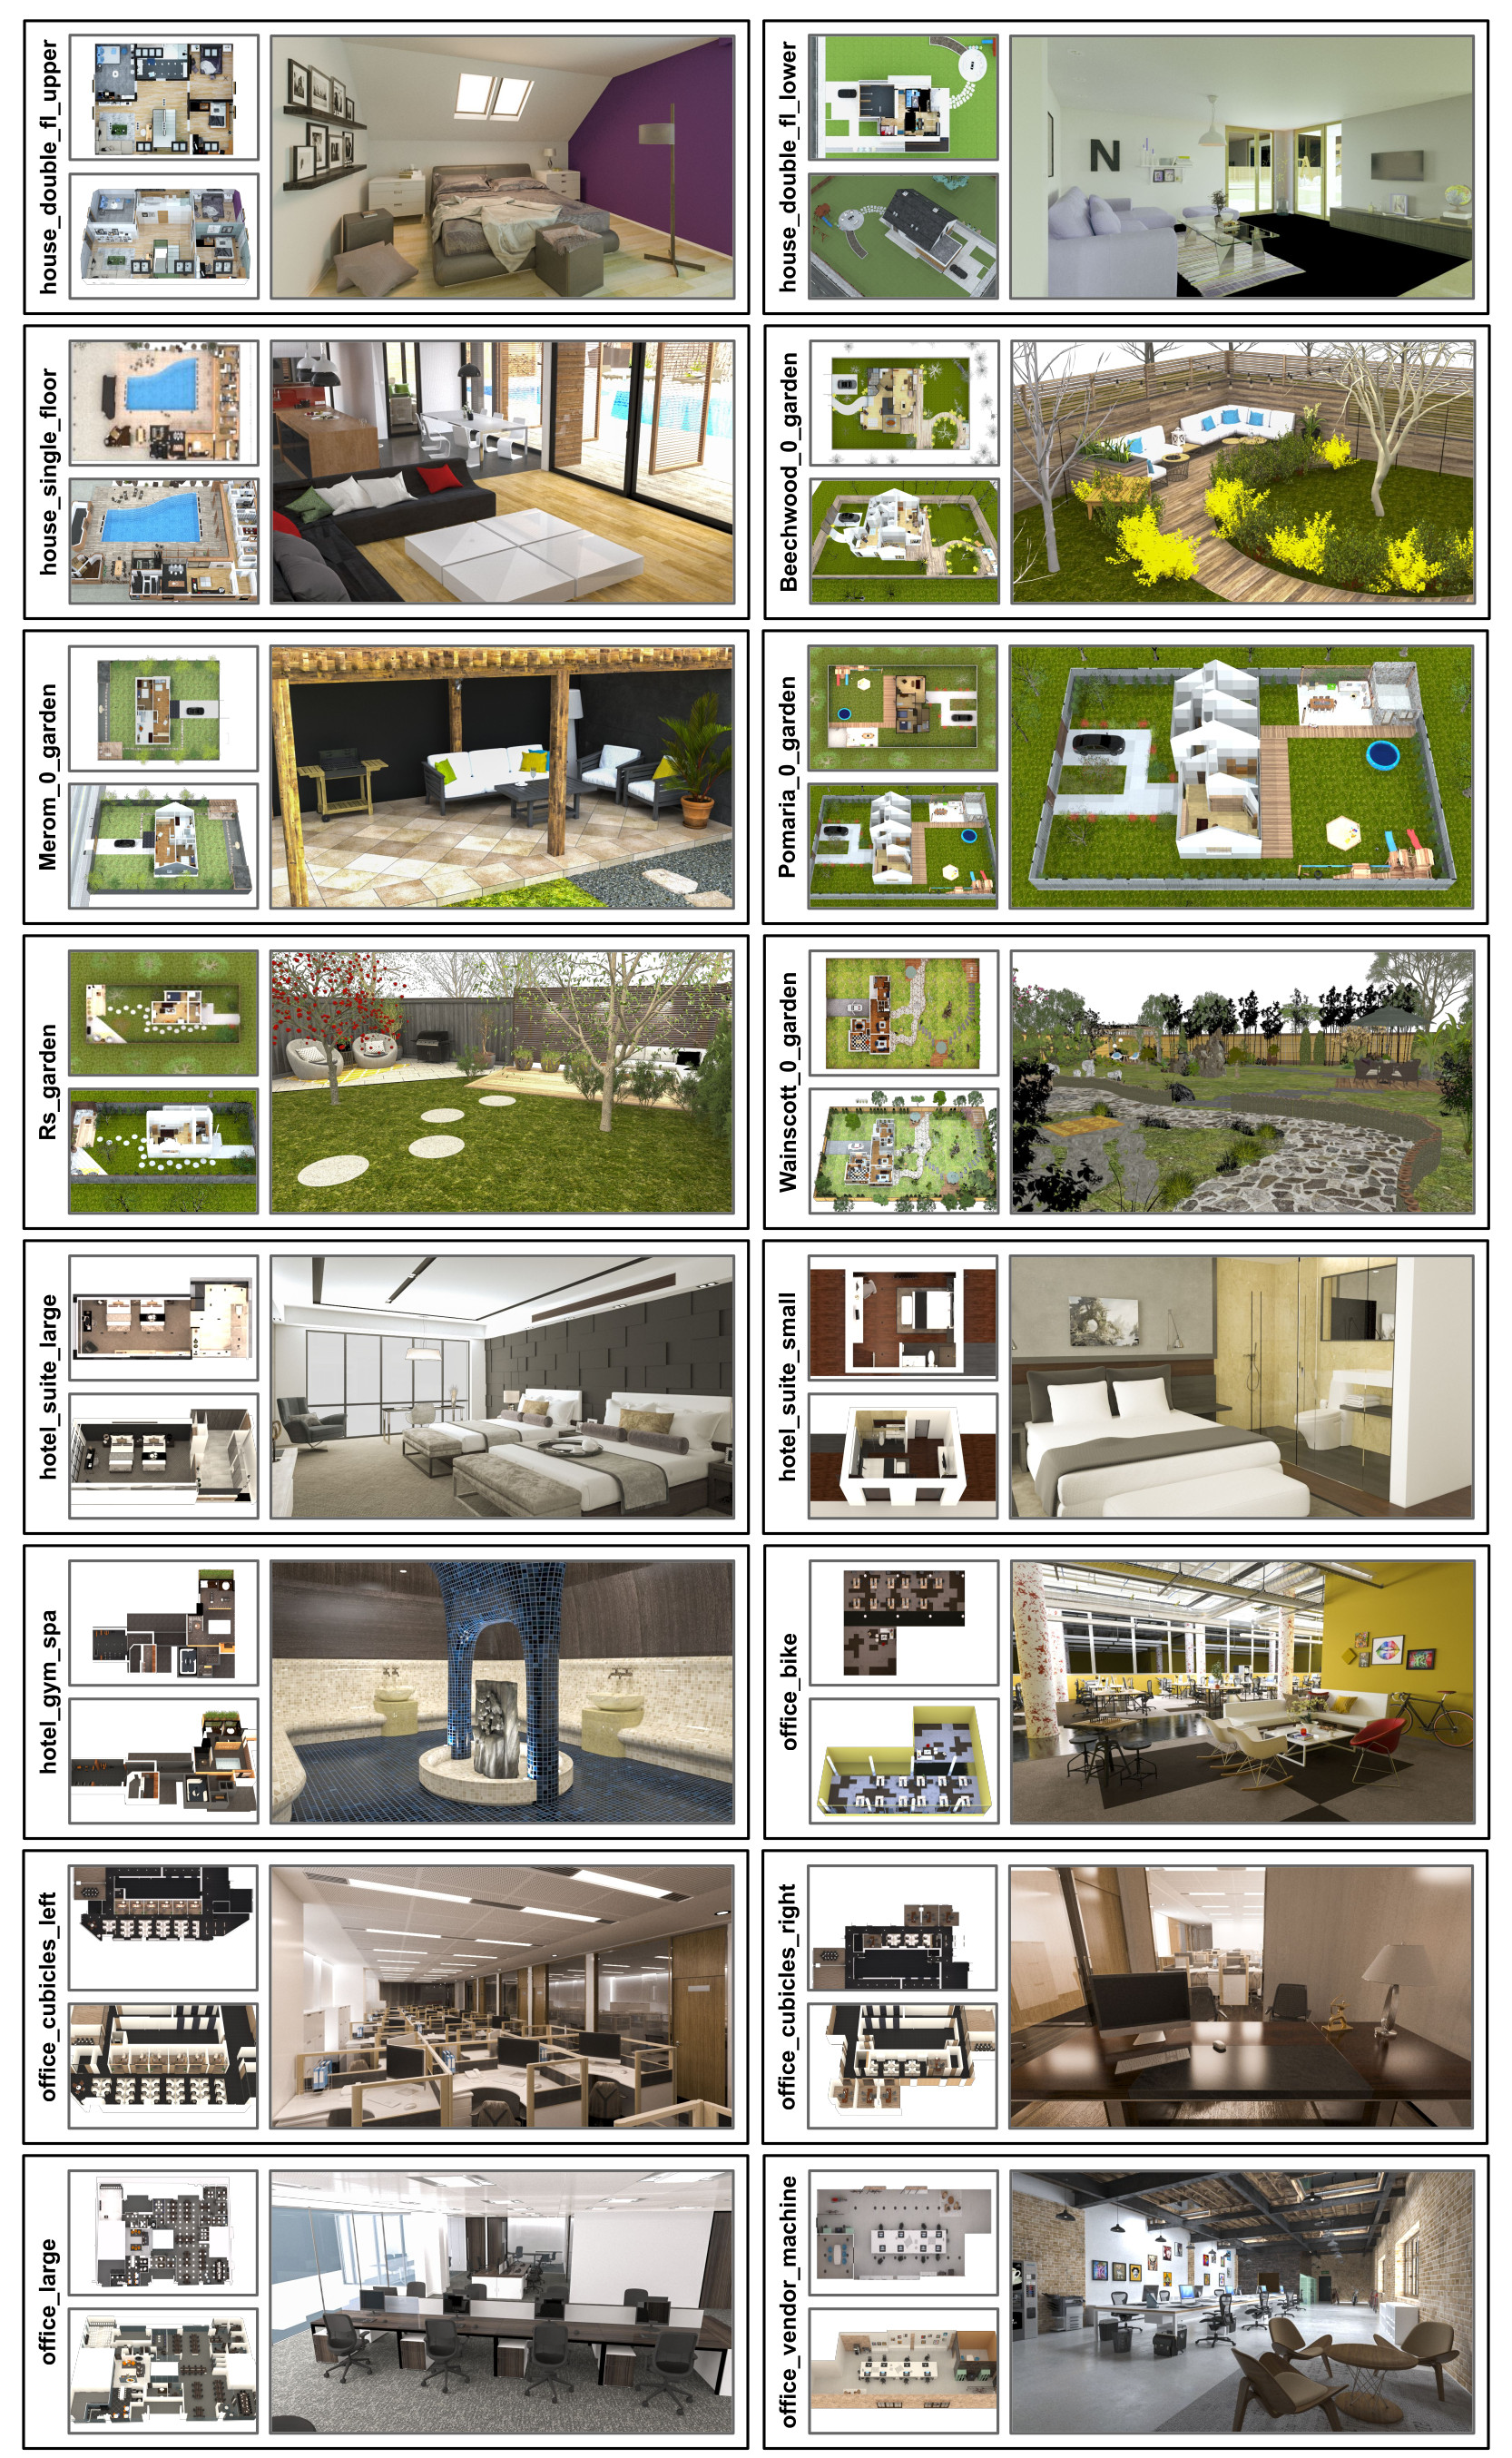
\includegraphics[width=\textwidth]{figures/models/scene_collage_p1.jpg}
    \caption{\revision{Part 1 of a scene collage showing views of all 50 scenes.}}
    %\label{fig:model_scene}
\end{figure}

\begin{figure}[th!]
    \centering
    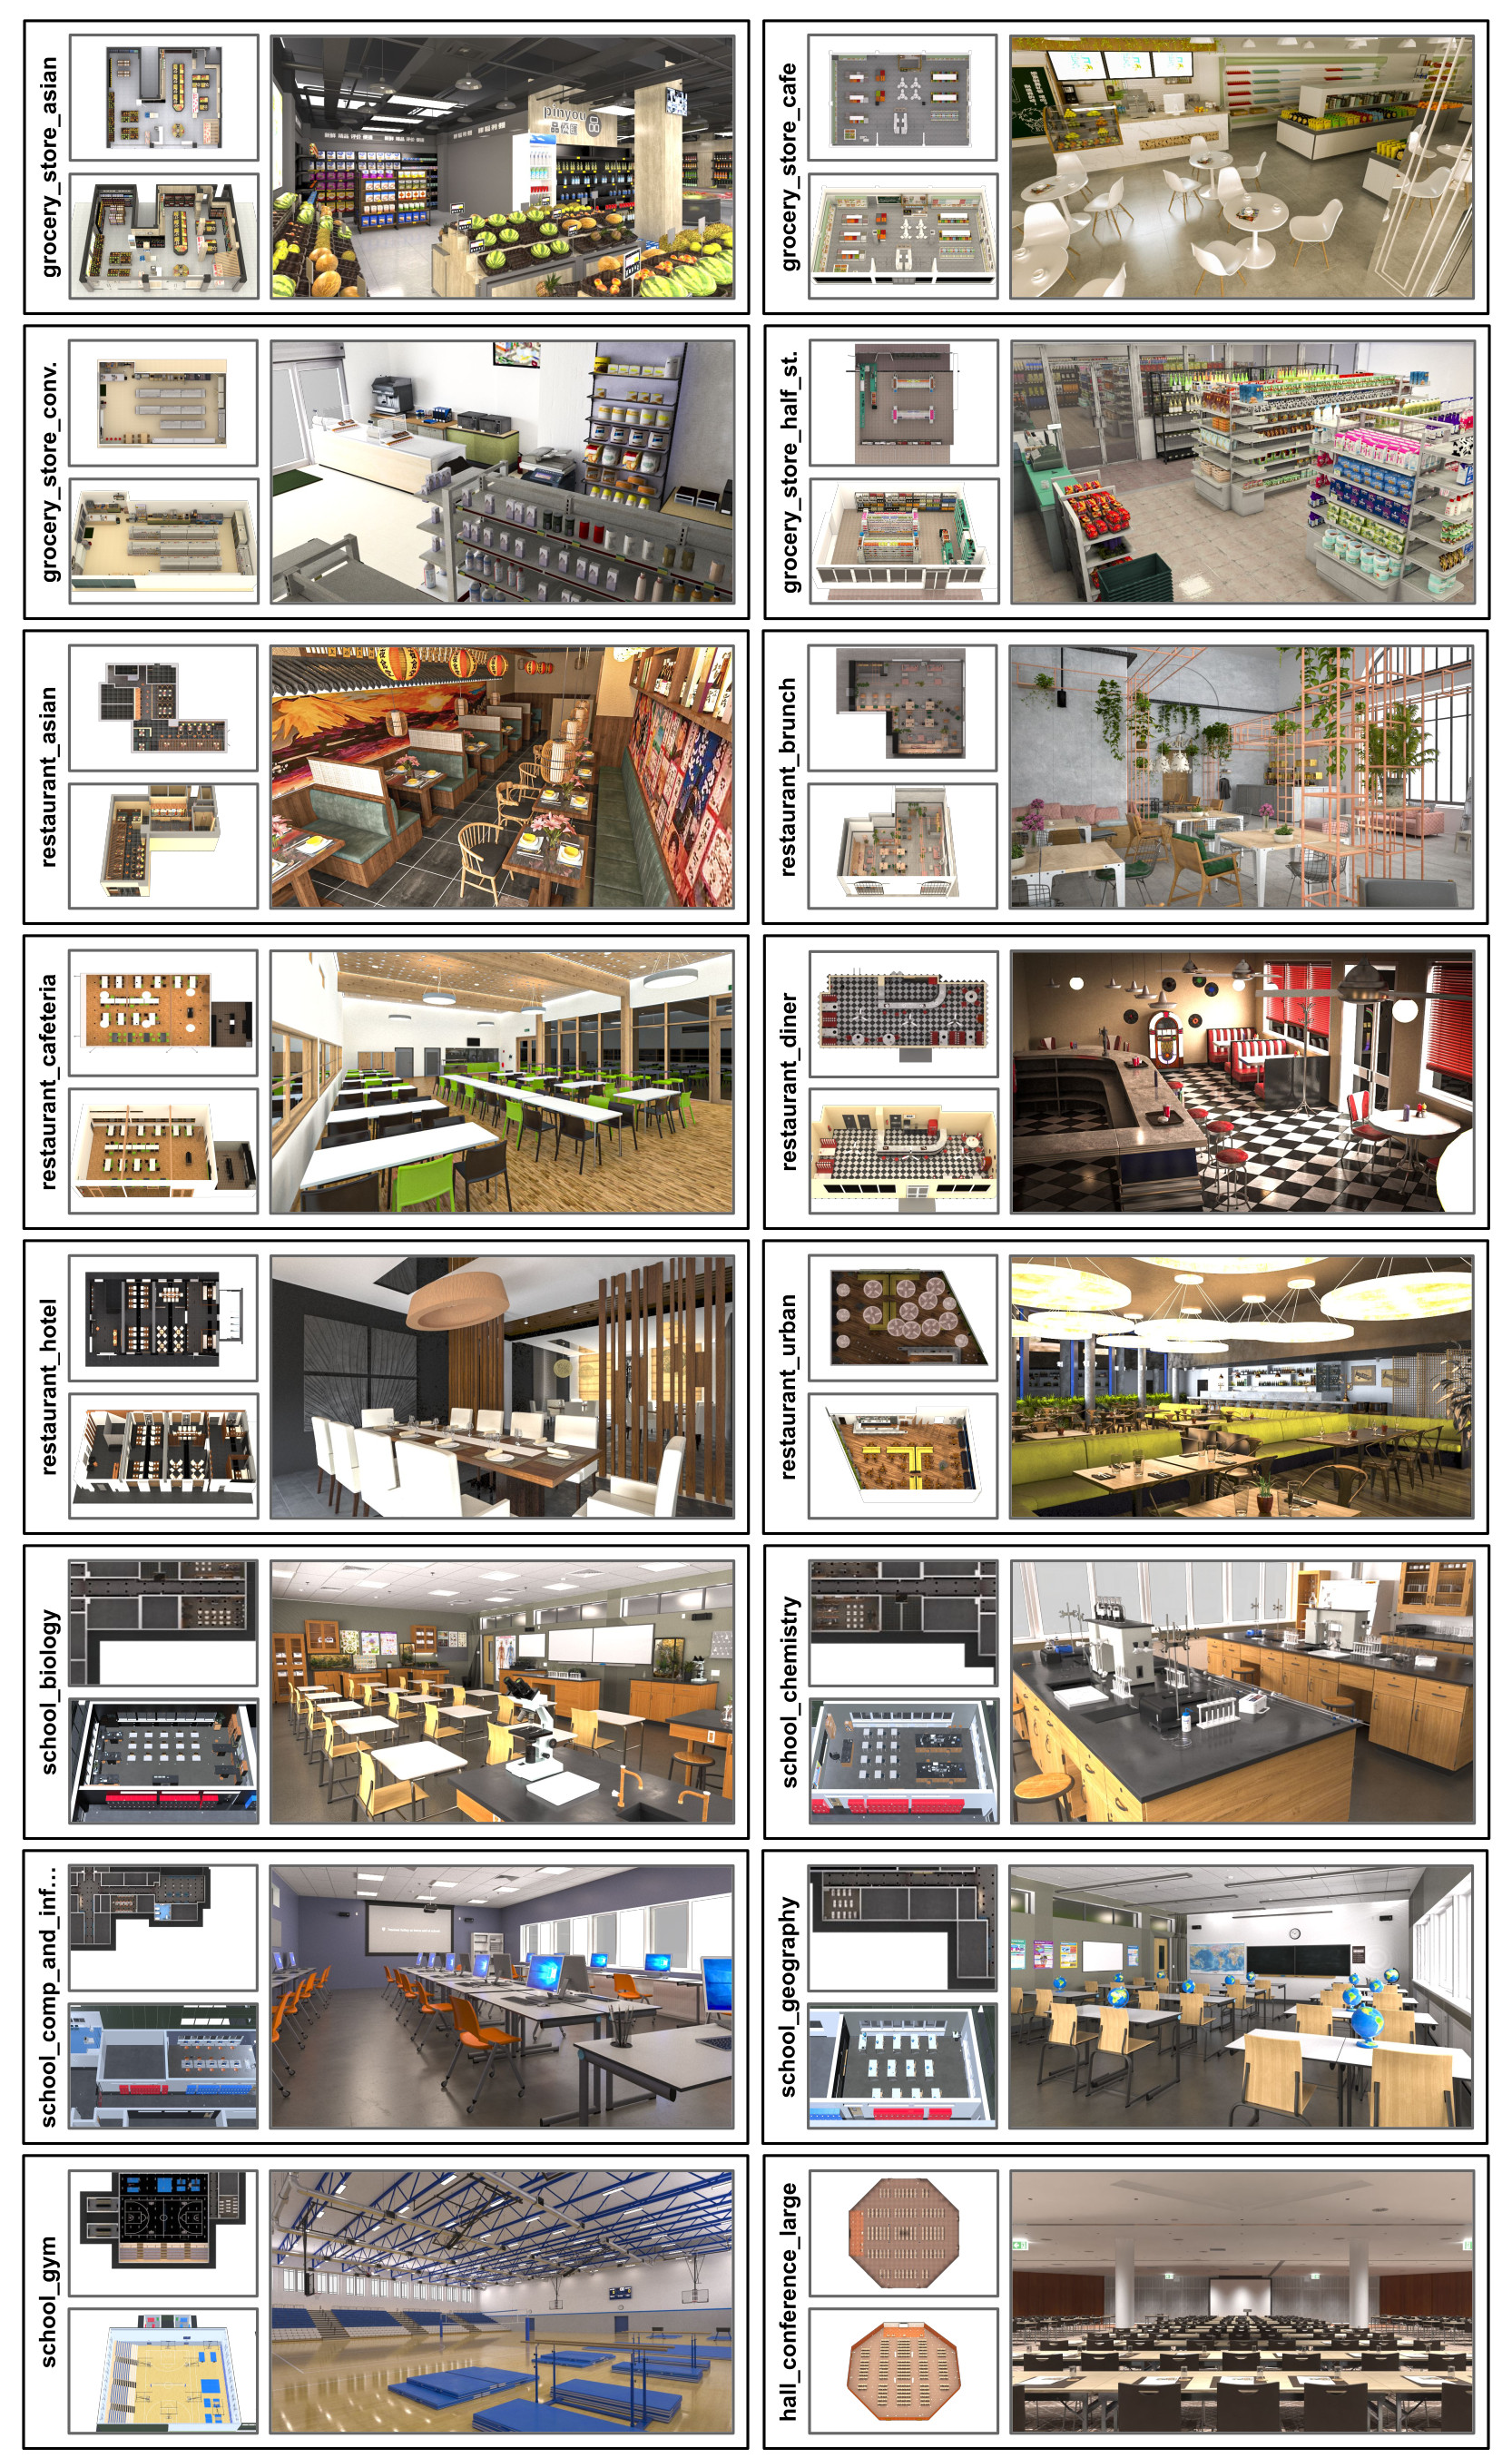
\includegraphics[width=\textwidth]{figures/models/scene_collage_p2.jpg}
    \caption{\revision{Part 2 of a scene collage showing views of all 50 scenes.}}
    %\label{fig:model_scene}
\end{figure}

\begin{figure}[th!]
    \centering
    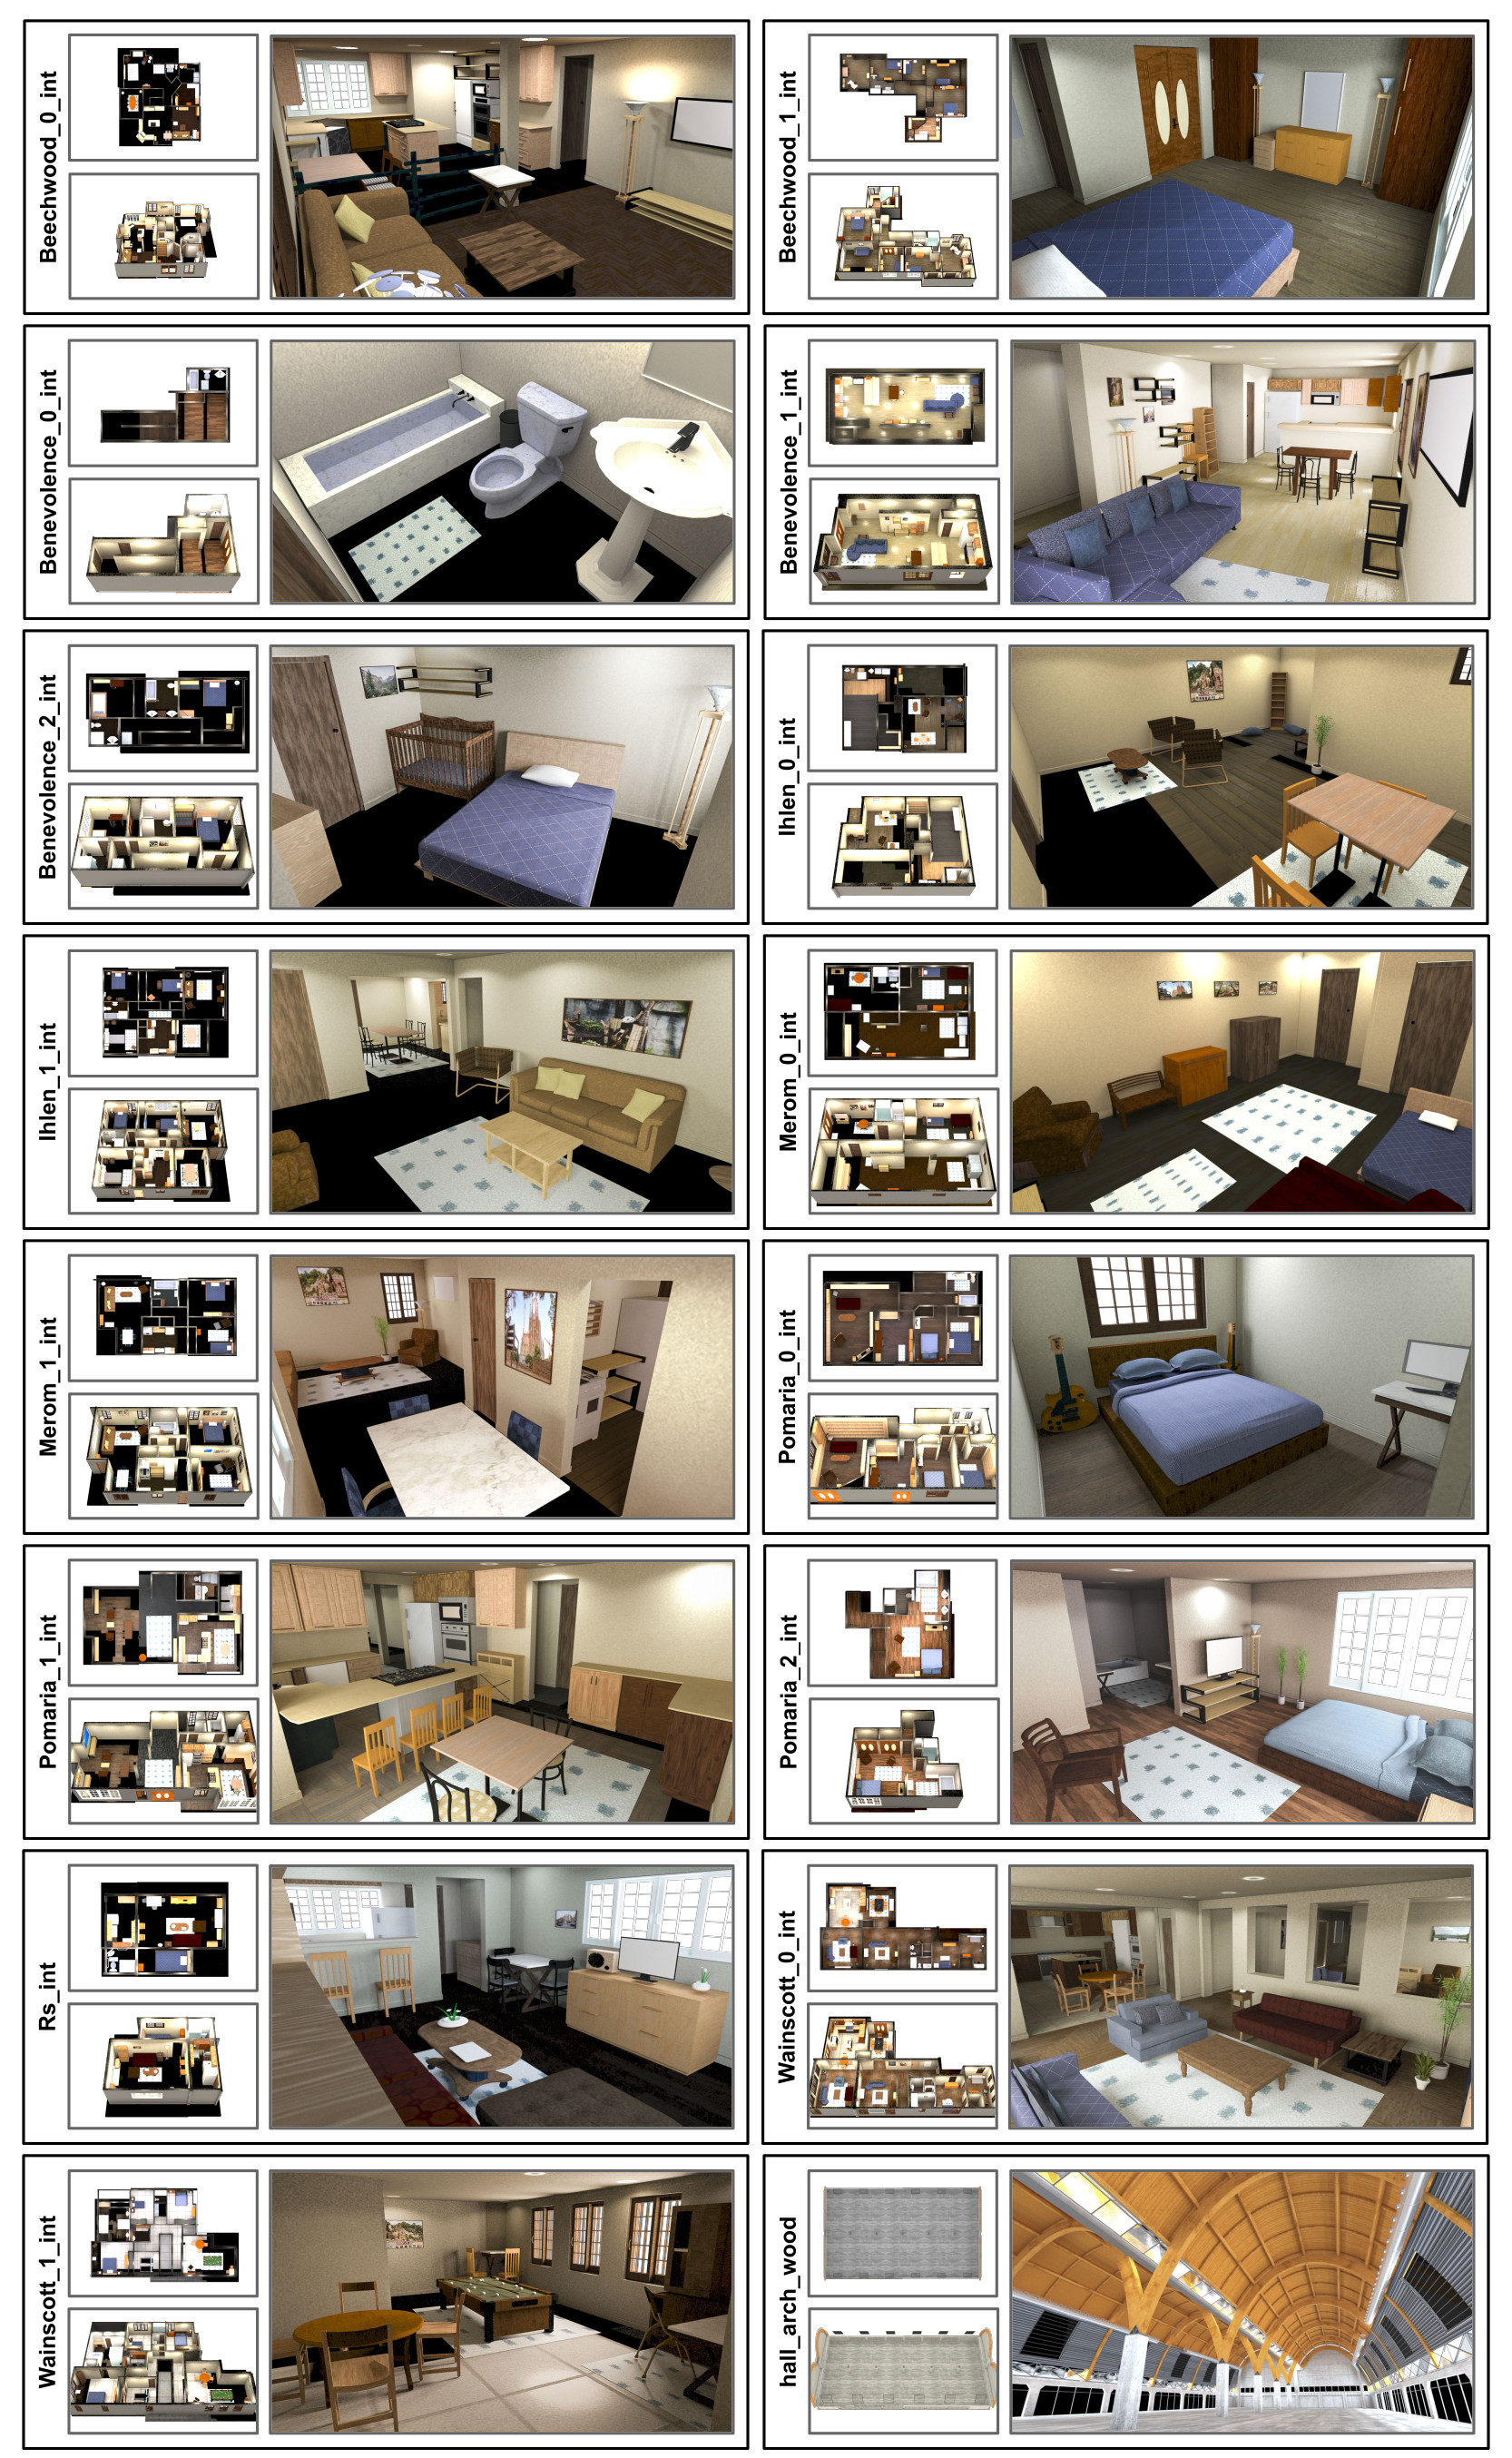
\includegraphics[width=\textwidth]{figures/models/scene_collage_p3.jpg}
    \caption{\revision{Part 3 of a scene collage showing views of all 50 scenes.}}
    %\label{fig:model_scene}
\end{figure}

\begin{figure}[th!]
    \centering
    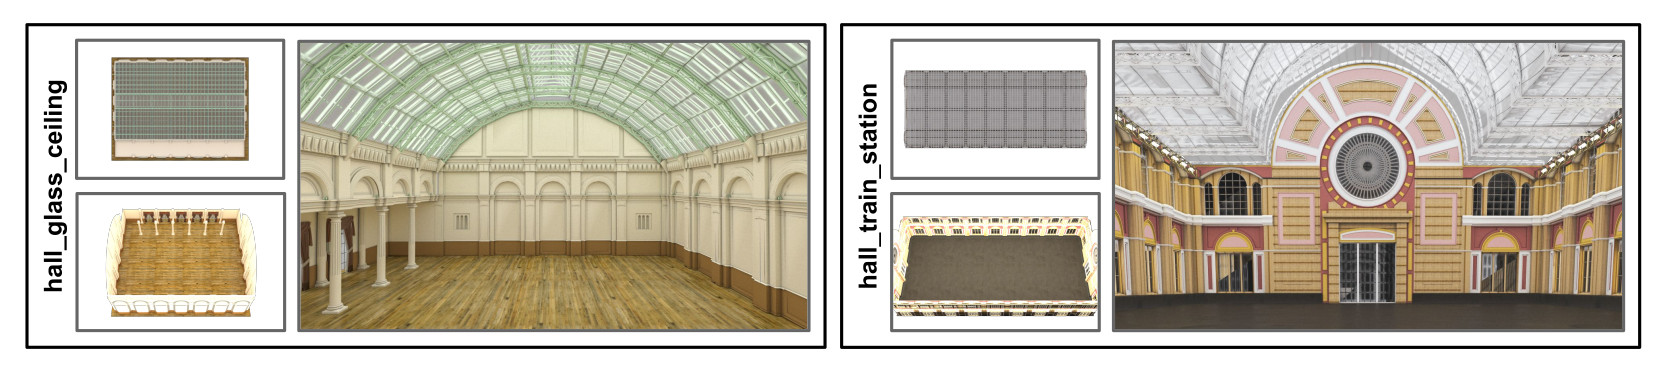
\includegraphics[width=\textwidth]{figures/models/scene_collage_p4.jpg}
    \caption{\revision{Part 4 of a scene collage showing views of all 50 scenes.}}
    %\label{fig:model_scene}
\end{figure}

\begin{figure}[th!]
 \centering
 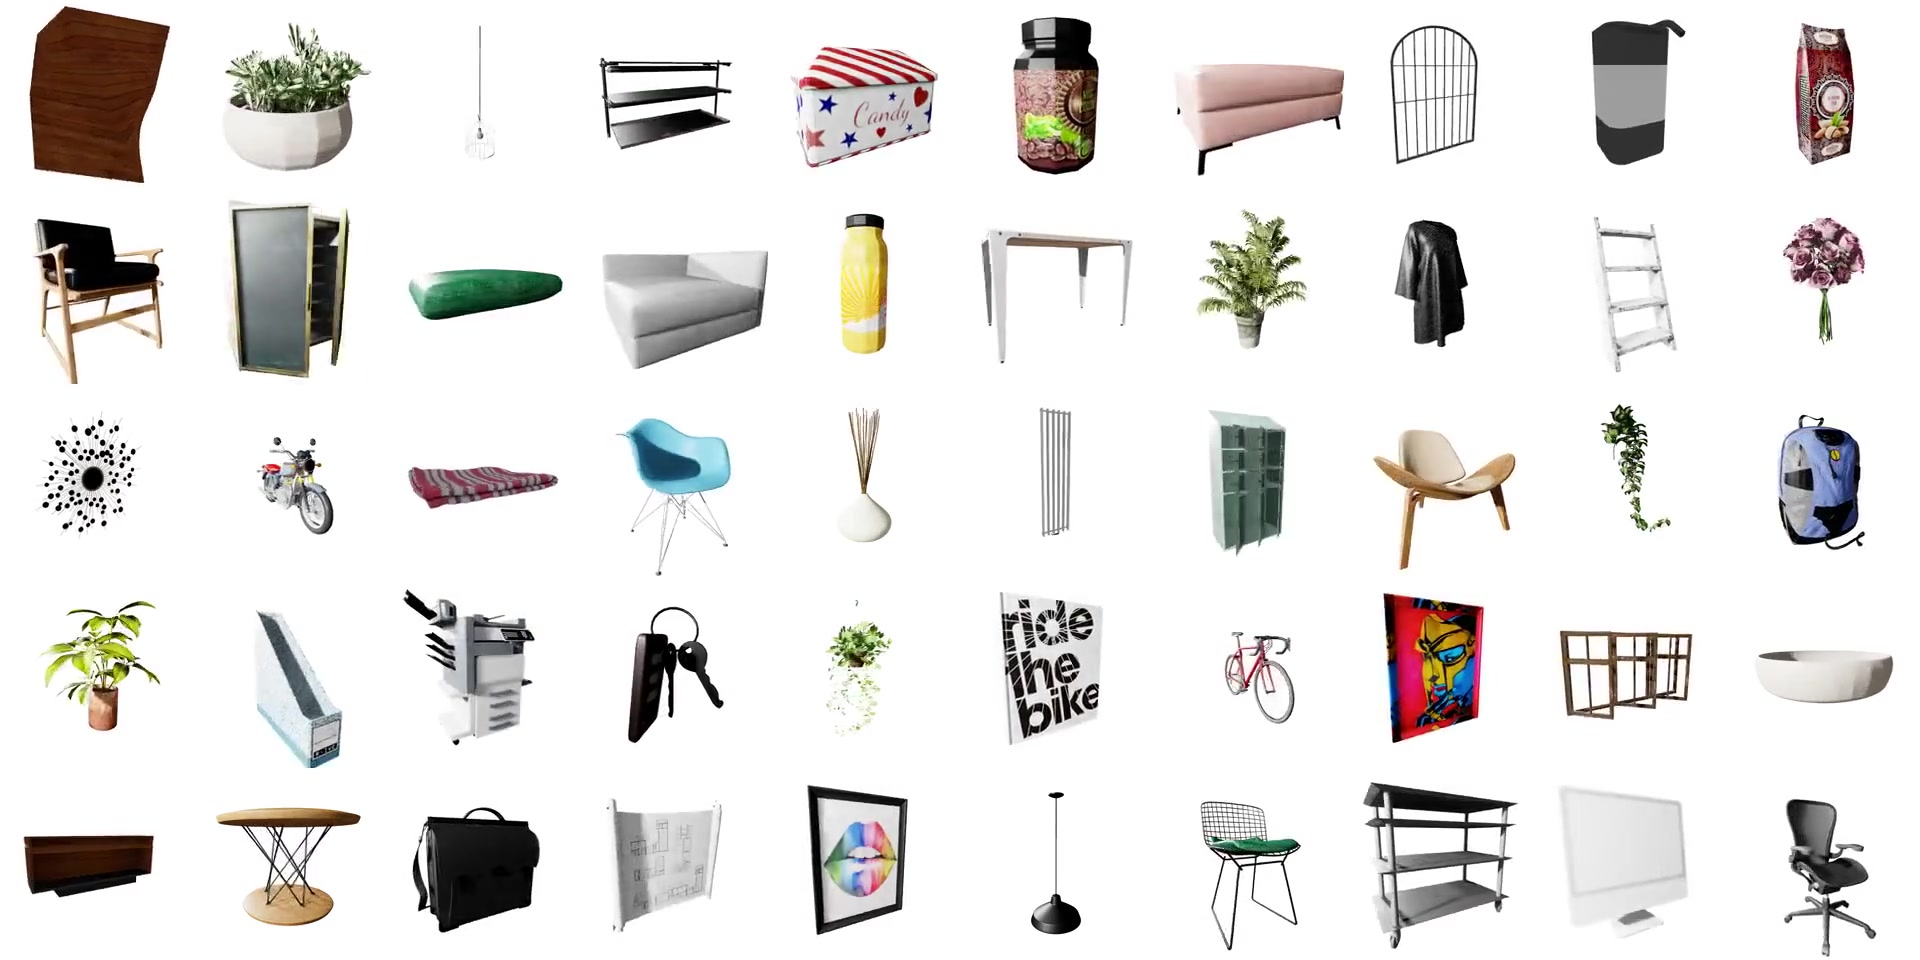
\includegraphics[width=0.9\textwidth]{figures/models/object_collage_3.jpg}
 \caption{\revision{A collage of objects included in the \dataset. These objects highlight key features of \simulator such as transparency, articulation, heat simulation, and lighting.}}
 \label{fig:model_object}
\end{figure}

\vspace{1.5cm}

{\scriptsize
\begin{longtable}{|m{.03\textwidth}|m{.16\textwidth}|m{.02\textwidth}|m{.02\textwidth}|m{.02\textwidth}|m{.27\textwidth}|m{.27\textwidth}|}
\hline
Scene Type
& Scene Name                            & Obj. Cnt.    & Syn. Cnt.    & Rm. Cnt.   & Room Types                                                                                                                                       & Example Activities                                                                                                                                                                                                                 \\ \hline
\multirow{15}{*}{\rotatebox[origin=c]{90}{\textbf{BEHAVIOR-100 Houses}}}
& Beechwood\_0\_int                     & 136          & 32           & 8          & \texttt{bathroom}, \texttt{corridor}, \texttt{dining\_room}, \texttt{entryway}, \texttt{kitchen}, \texttt{living\_room}, \texttt{private\_office}, \texttt{utility\_room}                                                & \texttt{clean a hot water dispenser}, \texttt{freeze lasagna}, \texttt{clean batting gloves}      \\ \cline{2-7} 
& Beechwood\_1\_int                     & 129          & 21           & 9          & \texttt{bathroom}, \texttt{bedroom}, \texttt{childs\_room}, \texttt{closet}, \texttt{corridor}, \texttt{playroom}, \texttt{television\_room }                                                                   & \texttt{clean your kitty litter box}, \texttt{store baby clothes}, \texttt{cleaning pet bed}      \\ \cline{2-7} 
& Benevolence\_0\_int                   & 21           & 10           & 4          & \texttt{bathroom}, \texttt{corridor}, \texttt{empty\_room}, \texttt{entryway}                                                                                                        & \texttt{laying clothes out}, \texttt{pack a pencil case}, \texttt{sweeping outside entrance}      \\ \cline{2-7} 
& Benevolence\_1\_int                   & 74           & 22           & 5          & \texttt{corridor}, \texttt{dining\_room}, \texttt{kitchen}, \texttt{living\_room}, \texttt{storage\_room}                                                                                     & \texttt{hanging blinds}, \texttt{sorting volunteer materials}, \texttt{wash baby bottles}      \\ \cline{2-7} 
& Benevolence\_2\_int                   & 63           & 23           & 5          & \texttt{bathroom}, \texttt{bedroom}, \texttt{corridor}                                                                                                                      & \texttt{clean walls}, \texttt{washing fabrics}, \texttt{folding clean laundry}      \\ \cline{2-7} 
& Ihlen\_0\_int                         & 68           & 21           & 7          & \texttt{bathroom}, \texttt{corridor}, \texttt{dining\_room}, \texttt{garage}, \texttt{living\_room}, \texttt{storage\_room}                                                                            & \texttt{de-clutter your garage}, \texttt{sorting household items}, \texttt{set up a home office in your garage}      \\ \cline{2-7} 
& Ihlen\_1\_int                         & 147          & 27           & 9          & \texttt{bathroom}, \texttt{bedroom}, \texttt{corridor}, \texttt{dining\_room}, \texttt{kitchen}, \texttt{living\_room}, \texttt{staircase}                                                                      & \texttt{clean jewels}, \texttt{clean green beans}, \texttt{hanging up curtains}      \\ \cline{2-7} 
& Merom\_0\_int                         & 82           & 27           & 6          & \texttt{bathroom}, \texttt{childs\_room}, \texttt{living\_room}, \texttt{playroom}, \texttt{storage\_room}, \texttt{utility\_room}                                                                     & \texttt{changing dog's water}, \texttt{wash a bra}, \texttt{wash a wool coat}      \\ \cline{2-7} 
& Merom\_1\_int                         & 123          & 28           & 8          & \texttt{bathroom}, \texttt{bedroom}, \texttt{childs\_room}, \texttt{corridor}, \texttt{dining\_room}, \texttt{kitchen}, \texttt{living\_room}, \texttt{staircase}                                                        & \texttt{store an uncooked turkey}, \texttt{drying table}, \texttt{clean flip flops}      \\ \cline{2-7} 
& Pomaria\_0\_int                       & 71           & 22           & 6          & \texttt{bathroom}, \texttt{bedroom}, \texttt{corridor}, \texttt{private\_office}, \texttt{television\_room }                                                                                  & \texttt{prepare sea salt soak}, \texttt{clean sheets}, \texttt{dispose of medication}      \\ \cline{2-7} 
& Pomaria\_1\_int                       & 89           & 24           & 6          & \texttt{bathroom}, \texttt{corridor}, \texttt{kitchen}, \texttt{living\_room}, \texttt{pantry\_room}, \texttt{utility\_room}                                                                           & \texttt{store brownies}, \texttt{clean a book}, \texttt{baking sugar cookies}      \\ \cline{2-7} 
& Pomaria\_2\_int                       & 42           & 18           & 3          & \texttt{bathroom}, \texttt{bedroom}, \texttt{corridor}                                                                                                                      & \texttt{replacing screens}, \texttt{clean baby toys}, \texttt{putting up posters}      \\ \cline{2-7} 
& Rs\_int                               & 72           & 32           & 5          & \texttt{bathroom}, \texttt{bedroom}, \texttt{entryway}, \texttt{kitchen}, \texttt{living\_room}                                                                                               & \texttt{dispose of a pizza box}, \texttt{putting food in fridge}, \texttt{putting out condiments}      \\ \cline{2-7} 
& Wainscott\_0\_int                     & 187          & 35           & 9          & \texttt{bathroom}, \texttt{bedroom}, \texttt{dining\_room}, \texttt{kitchen}, \texttt{living\_room}                                                                                           & \texttt{make microwave popcorn}, \texttt{make frozen lemonade}, \texttt{make cake mix}      \\ \cline{2-7} 
& Wainscott\_1\_int                     & 150          & 26           & 10         & \texttt{bathroom}, \texttt{bedroom}, \texttt{corridor}, exercise\_room, \texttt{playroom}, \texttt{private\_office}, \texttt{utility\_room}                                                            & \texttt{decorating for religious ceremony}, \texttt{stash snacks in your room}, \texttt{disinfect laundry}      \\ \hline
\multirow{5}{*}{\rotatebox[origin=c]{90}{{\textbf{BEHAVIOR-100 Houses+Garden}}}}
& Beechwood\_0\_garden                  & 335          & 45           & 9          & \texttt{bathroom}, \texttt{corridor}, \texttt{dining\_room}, \texttt{entryway}, \texttt{garden}, \texttt{kitchen}, \texttt{living\_room}, \texttt{private\_office}, \texttt{utility\_room}                                        & \texttt{tidy your garden}, \texttt{opening doors}, \texttt{wash goalkeeper gloves}      \\ \cline{2-7} 
& Merom\_0\_garden                      & 197          & 51           & 8          & \texttt{bathroom}, \texttt{childs\_room}, \texttt{garden}, \texttt{living\_room}, \texttt{playroom}, \texttt{sauna}, \texttt{storage\_room}, \texttt{utility\_room}                                                      & \texttt{clean your kitty litter box}, \texttt{clean a glass windshield}, \texttt{hang icicle lights}      \\ \cline{2-7} 
& Pomaria\_0\_garden                    & 260          & 49           & 7          & \texttt{bathroom}, \texttt{bedroom}, \texttt{corridor}, \texttt{garden}, \texttt{private\_office}, \texttt{television\_room }                                                                          & \texttt{putting up Christmas lights outside}, \texttt{prepare a hanging basket}, \texttt{clean a patio}      \\ \cline{2-7} 
& Rs\_garden                            & 185          & 47           & 6          & \texttt{bathroom}, \texttt{bedroom}, \texttt{entryway}, \texttt{garden}, \texttt{kitchen}, \texttt{living\_room}                                                                                       & \texttt{cleaning driveway}, \texttt{clean a longboard}, \texttt{roast nuts}      \\ \cline{2-7} 
& Wainscott\_0\_garden                  & 712          & 61           & 10         & \texttt{bathroom}, \texttt{bedroom}, \texttt{dining\_room}, \texttt{garden}, \texttt{kitchen}, \texttt{living\_room}                                                                                   & \texttt{clean an espresso machine}, \texttt{clearing food from table into fridge}, \texttt{painting porch}      \\ \hline
\multirow{3}{*}{\rotatebox[origin=c]{90}{\textbf{New Houses}}}
& house\_single\_floor                  & 1375         & 137          & 23         & \texttt{bathroom}, \texttt{bedroom}, \texttt{childs\_room}, \texttt{closet}, \texttt{corridor}, \texttt{dining\_room}, \texttt{empty\_room}, \texttt{entryway}, \texttt{garden}, \texttt{kitchen}, \texttt{living\_room}, \texttt{sauna}, \texttt{utility\_room}      & \texttt{turning out all lights before sleep}, \texttt{iron curtains}, \texttt{packing hobby equipment}      \\ \cline{2-7} 
& {\tiny house\_double\_floor\_lower}   & 304          & 79           & 6          & \texttt{bathroom}, \texttt{corridor}, \texttt{garage}, \texttt{garden}, \texttt{kitchen}, \texttt{living\_room}                                                                                        & \texttt{wash towels}, \texttt{clean a fish}, \texttt{clean brass}      \\ \cline{2-7} 
& {\tiny house\_double\_floor\_upper}   & 325          & 78           & 5          & \texttt{bathroom}, \texttt{bedroom}, \texttt{television\_room }                                                                                                             & \texttt{clean a saxophone}, \texttt{taking down curtains}, \texttt{clean walls}      \\ \hline
\multirow{4}{*}{\rotatebox[origin=c]{90}{\textbf{Grocery Stores}}}
& grocery\_store\_asian                 & 3402         & 79           & 2          & \texttt{bathroom}, \texttt{grocery\_store}                                                                                                                         & \texttt{buy alcohol}, \texttt{buy boxes for packing}, \texttt{buy a microwave oven}      \\ \cline{2-7} 
& grocery\_store\_cafe                  & 6994         & 71           & 4          & \texttt{bar} , \texttt{bathroom}, \texttt{dining\_room}, \texttt{grocery\_store}                                                                                                      & \texttt{defrost meat}, \texttt{clean reusable shopping bags}, \texttt{buy a good avocado}      \\ \cline{2-7} 
& {\tiny grocery\_store\_convenience}   & 1889         & 82           & 2          & \texttt{bathroom}, \texttt{grocery\_store}                                                                                                                         & \texttt{washing windows}, \texttt{picking up prescriptions}, \texttt{buy food for vegetarians}      \\ \cline{2-7} 
& {\tiny grocery\_store\_half\_stocked} & 3804         & 51           & 2          & \texttt{bathroom}, \texttt{grocery\_store}                                                                                                                         & \texttt{buying gardening supplies}, \texttt{buy basic garden tools}, \texttt{buy boxes for packing}      \\ \hline
\multirow{4}{*}{\rotatebox[origin=c]{90}{\textbf{Halls}}}
& hall\_arch\_wood                      & 78           & 11           & 2          & \texttt{bathroom}, \texttt{empty\_room}                                                                                                                         &    \texttt{clean walls}  \\ \cline{2-7} 
& hall\_train\_station                  & 141          & 15           & 2          & \texttt{bathroom}, \texttt{empty\_room}                                                                                                                            &  \texttt{clean cement}    \\ \cline{2-7} 
& hall\_glass\_ceiling                  & 116          & 20           & 2          & \texttt{bathroom}, \texttt{empty\_room}                                                                                                                            &  \texttt{preparing food for a fundraiser}   \\ \cline{2-7} 
& hall\_conference\_large               & 3372         & 26           & 2          & \texttt{bathroom}, \texttt{conference\_hall}                                                                                                                       &  \texttt{distributing event T-shirts}    \\ \hline
\multirow{3}{*}{\rotatebox[origin=c]{90}{\textbf{Hotels}}}
& hotel\_gym\_spa                       & 322          & 43           & 9          & \texttt{bathroom}, \texttt{corridor}, \texttt{gym} , \texttt{hammam} , \texttt{locker\_room} , \texttt{sauna}, \texttt{spa}                                                                                         & \texttt{turning on the hot tub}, \texttt{adding chemicals to hot tub}, \texttt{clean a sauna}      \\ \cline{2-7}
& hotel\_suite\_large                   & 218          & 51           & 2          & \texttt{bathroom}, \texttt{bedroom}                                                                                                                                & \texttt{clean vinyl shutters}, \texttt{cleaning computer}, \texttt{clean white marble}      \\ \cline{2-7} 
& hotel\_suite\_small                   & 48           & 28           & 2          & \texttt{bathroom}, \texttt{bedroom}                                                                                                                                & \texttt{clean cork mats}, \texttt{putting out clean towels}, \texttt{clean a shower}      \\ \hline
\multirow{5}{*}{\rotatebox[origin=c]{90}{\textbf{Offices}}}
& office\_bike                          & 479          & 49           & 3          & \texttt{bathroom}, \texttt{break\_room}, \texttt{shared\_office}                                                                                                            & \texttt{set up a webcam}, \texttt{set up two computer monitors}, \texttt{clean an office chair}      \\ \cline{2-7} 
& office\_cubicles\_left                & 787          & 44           & 12         & \texttt{bathroom}, \texttt{conference\_hall}, \texttt{copy\_room}, \texttt{corridor}, \texttt{lobby}, \texttt{meeting\_room}, \texttt{private\_office}, \texttt{shared\_office}                                          & \texttt{clean up your desk}, \texttt{clean a LED screen}, \texttt{laying out snacks at work}      \\ \cline{2-7} 
& office\_cubicles\_right               & 406          & 37           & 11         & \texttt{bathroom}, \texttt{conference\_hall}, \texttt{copy\_room}, \texttt{corridor}, \texttt{lobby}, \texttt{meeting\_room}, \texttt{private\_office}, \texttt{shared\_office}                                          & \texttt{making photocopies}, \texttt{clean a LED screen}, \texttt{clean a keyboard}      \\ \cline{2-7} 
& office\_large                         & 1151         & 46           & 24         & \texttt{bathroom}, \texttt{break\_room}, \texttt{conference\_hall}, \texttt{copy\_room}, \texttt{corridor}, \texttt{lobby}, \texttt{meeting\_room}, \texttt{phone\_room}, \texttt{private\_office}, \texttt{shared\_office}                & \texttt{emptying trash cans}, \texttt{putting meal in fridge at work}, \texttt{brewing coffee}      \\ \cline{2-7} 
& office\_vendor\_machine               & 225          & 45           & 4          & \texttt{bathroom}, \texttt{break\_room}, \texttt{meeting\_room}, \texttt{shared\_office}                                                                                             & \texttt{clean a computer monitor}, \texttt{make the workplace exciting}, \texttt{dispose of glass}      \\ \hline
\multirow{6}{*}{\rotatebox[origin=c]{90}{\textbf{Restaurants}}}
& restaurant\_asian                     & 1221         & 56           & 3          & \texttt{bathroom}, \texttt{dining\_room}, \texttt{kitchen}                                                                                                                  & \texttt{grill vegetables}, \texttt{cook tofu}, \texttt{clean clams}      \\ \cline{2-7} 
& restaurant\_brunch                    & 1096         & 70           & 4          & \texttt{bar} , \texttt{bathroom}, \texttt{dining\_room}, \texttt{kitchen}                                                                                                             & \texttt{stock a bar}, \texttt{cook squid}, \texttt{washing vegetables}      \\ \cline{2-7} 
& restaurant\_cafeteria                 & 292          & 45           & 3          & \texttt{bathroom}, \texttt{dining\_room}, \texttt{kitchen}                                                                                                                  & \texttt{clean a popcorn machine}, \texttt{store coffee beans or ground coffee}, \texttt{roast meat}      \\ \cline{2-7} 
& restaurant\_diner                     & 174          & 39           & 3          & \texttt{bar} , \texttt{bathroom}, \texttt{dining\_room}                                                                                                                      & \texttt{sweeping floors}, \texttt{installing smoke detectors}, \texttt{clean a lobster}      \\ \cline{2-7} 
& restaurant\_hotel                     & 1080         & 81           & 4          & \texttt{bathroom}, \texttt{dining\_room}, \texttt{kitchen}, \texttt{lobby}                                                                                                           & \texttt{clean eggs}, \texttt{setting table for coffee}, \texttt{clean a pizza stone}      \\ \cline{2-7}
& restaurant\_urban                     & 1368         & 90           & 4          & \texttt{bar} , \texttt{bathroom}, \texttt{dining\_room}, \texttt{kitchen}                                                                                                             & \texttt{cook pumpkin seeds}, \texttt{putting roast in oven}, \texttt{thaw frozen fish}      \\ \hline
\multirow{5}{*}{\rotatebox[origin=c]{90}{\textbf{Schools}}}
& school\_biology                       & 717          & 53           & 4          & \texttt{bathroom}, \texttt{biology\_lab} , \texttt{corridor}                                                                                                                 & \texttt{clean an eraser}, \texttt{turning sprinkler off}, \texttt{clean a glass pipe}      \\ \cline{2-7} 
& school\_chemistry                     & 890          & 69           & 4          & \texttt{bathroom}, \texttt{chemistry\_lab} , \texttt{corridor}                                                                                                               & \texttt{clean clear plastic}, \texttt{clean an eraser}, \texttt{clean a whiteboard}      \\ \cline{2-7} 
& {\tiny school\_comp\_lab\_infirmary}  & 828          & 61           & 6          & \texttt{bathroom}, \texttt{computer\_lab}, \texttt{corridor}, \texttt{infirmary}                                                                                                     & \texttt{clean a computer monitor}, \texttt{prepare an emergency school kit}, \texttt{clean a keyboard}      \\ \cline{2-7} 
& school\_geography                     & 556          & 42           & 5          & \texttt{bathroom}, \texttt{classroom}, \texttt{corridor}                                                                                                                    & \texttt{clean gold}, \texttt{clean a glass pipe}, \texttt{clean an eraser}      \\ \cline{2-7} 
& school\_gym                           & 853          & 36           & 7          & \texttt{bathroom}, \texttt{corridor}, \texttt{gym} , \texttt{locker\_room}                                                                                                             & \texttt{clean a dirty baseball}, \texttt{dispose of glass}, \texttt{wash towels}      \\ \hline

\caption{Statistics and information for each of 50 scenes in B1K: scene type, name, number of objects, unique synsets and rooms, room types, and example activities }
\label{tab:model_scene}
\end{longtable}
}




% Furthermore, the diversity of the activities in our new environments (such as cleaning in offices, or cooking in restaurants) requires certain types of rooms (e.g. public restrooms and commercial kitchens) to be present in the scenes, which is not typically the case for available models. To support these use cases, 5 public restroom models and 2 commercial kitchen models were separately acquired from Turbosquid, and attached to non-house scenes as necessary, with pairings being made based on visual compatibility. The seamless integration of these partial scenes into the larger scenes also allows the reuse of objects across the scenes while still representing the diversity of such environments. Another important requirement that arose from the survey results was that the participants consistently want robots to help with outdoor activities (e.g. gardening, shoveling snow, etc.), which cannot be simulated in the indoor-only \oldbenchmark scenes. To resolve this, the \dataset contains both entirely new houses that have gardens, as well as augmented versions of \oldbenchmark houses that have gardens attached. These gardens, diverse in terms of both size and features, were also separately acquired from TurboSquid, and were attached to the house scenes by professional architects that were contracted on Upwork. Exterior walls were also added to the previously indoor-only houses, representing a variety of architectural styles that are prevalent globally.


% To be imported into \simulator, scene and object models that were acquired from online marketplaces were processed by members of our team through a purpose-built annotation process in Autodesk 3ds Max, designed to correctly label each object's articulations, lights, and other features such as heating and toggling, as well as scene features such as room boundaries. Accurate labeling of canonical orientations and equally-granular categories (as well as whether certain objects should not be randomized) for each object, a critical requirement of the Object Randomization feature supported in \simulator, was also undertaken at this stage. The processed scene files were then run through our automated 3ds Max-to-\simulator pipeline, which exports the objects, their materials (including compatible features such as transparency and self-illumination), their joint configurations, and additional features as well as generating additional metadata (e.g. minimum-value bounding boxes) and checking for physics stability.